\chapter{绪论}\label{chap:introduction}

\section{电缆通道检测机器人的研究背景与意义}
近年来，城市基础设施与电力系统规模持续扩大，高压电缆通道的数量快速增加，分布也越来越广。电缆通道承担着电能输送和设备防护的核心任务，其运行状况直接影响到电力系统的安全稳定。但传统的人工巡检与验收方式，在实际应用中逐渐显露出几个方面的不足。

首先是作业效率偏低。人员需直接进入电缆通道开展验收，耗费大量人力物力；在面对长距离、多分支的电缆沟时，检测周期被明显拉长，效率很难得到保证。其次是安全风险较大。电缆通道大多为地下或有限空间环境，通风、照明条件较差，还可能出现有毒有害气体积聚、积水乃至局部塌方等危险，人工作业面临的不确定性和危险性都比较高。再次是数据精度有限。人工方式多依赖经验进行判断，难以对电缆沟内部的几何尺寸、构筑物形态、环境参数等实施高精度、全覆盖式的采集，漏检和误判的情况较难避免。

在电力运维日益向智能化、无人化方向发展的趋势下，研制适用于电缆通道的检测机器人，已成为破解上述难题的一条有效路径。这类机器人可以在狭窄且复杂的电缆沟内自主行走，利用搭载的多种传感器，同步完成结构尺寸测量、环境参数监测、缺陷识别及三维建模等工作，从而在效率、安全性和检测精度上为验收工作带来实质提升。

\section{电缆通道检测机器人方案选择}
本毕业设计在电缆通道检测机器人结构方案选择上，由于电缆通道中有台阶、错综复杂的电缆等障碍物，因此机器人需要具备基础的跨越障碍物功能。同时在电缆通道中不易更换电池，所以需要机器人具备高效率行驶的能力。在底盘方案中，常见轮式底盘满足高效行驶的能力，但无法跨越有高低地形差的障碍物；腿式底盘具备跨越障碍物的能力，但行驶速率较低。因此，本毕业设计综合两种底盘构型，选择轮腿式底盘进行后续运动控制仿真与路径规划模拟。

在运动控制方面，由于机器人腿部可以简化为倒立摆模型，常见倒立摆控制有pid控制和lqr控制，为同时控制各状态量，该系统为多输入多输出系统，因此本毕业设计选择lqr控制器进行运动控制仿真。

由于电缆通道中包含许多纵横交错的电缆、支架等静态障碍物，同时机器人需要具备躲避行进中人类的能力，因此检测对于路径规划的要求可基本简化为在一个具有复杂多样静态障碍物和动态障碍物的环境里导航到终点的问题。由于障碍物多变且复杂，机器人无提前建图的条件；在路径规划的过程中，机器人需要具备实时路径规划的能力。对于周围环境障碍物的感知，机器人采取雷达扫描的方式获取周围环境的障碍物情况，再进行实施路径规划。

传统路径规划算法主要有A*，DWA等，而A*算法需要完整的环境地图，且在动态环境中表现不佳；DWA算法虽然适用于动态环境，但其基于局部搜索，容易陷入局部最优解，且需要人工设计代价函数。相比之下，深度强化学习（DRL）算法能够通过与环境的交互学习到更符合任务目标的全局最优行为，具有自适应能力强、便于处理动态环境等优势。本毕业设计对比了DWA经典算法与深度强化学习的路径规划算法DQN、SAC进行仿真测试与优化，同时针对动态障碍物，串联Transfomer架构与SAC算法，提高算法针对动态障碍物的避障能力。另外，针对训练数据量大，训练时间长的问题，本毕业设计采用ASL训练架构，提高数据吞吐量，加速训练速度，。

\section{电缆通道检测机器人国内外研究现状}
\subsection{底盘结构方案：轮腿式底盘机器人}
2017年，Boston Dynamics公司曝光了一款轮式机器人Handle演示的视频\cite{BostonDynamics2012APA}，其最大特点是集轮子和腿为一体，兼具了轮式机器人和腿式机器人的优势。该机器人高约1.98m，重82kg，行进速度约14km/h，垂直跳跃高度约1.2m，一次充电的续航能力约为24km，可搬运45kg以上的重物，还能在多种恶劣环境下顺利行动，如山地,雪地和崎岖的地形。

\begin{figure}[htbp]
  \centering
  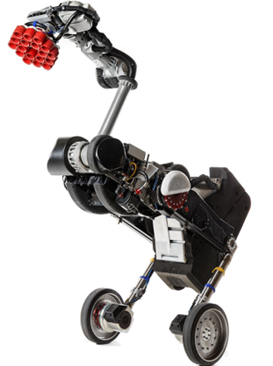
\includegraphics[width=0.5\textwidth,height=0.28\textheight,keepaspectratio]{figures/boston_handle.png}
  \caption{Boston Dynamics公司的轮腿式机器人Handle}
  \label{fig:boston-dynamics-handle}
\end{figure}
\FloatBarrier

苏黎世联邦理工（ETH Zurich）的学生团队Victor Klemm 等人于2018 年9 月研制出了名为Ascento 的双轮跳跃机器人，\cite{klemm2019ascento}该机器人主要用于室内巡检，平整地面用轮子快速移动，并通过跳跃来越障。机械结构方面Ascento腿部采用四连杆机构，使整车结构紧凑。Ascento 通过线性二次调节器 (LQR)实现机器人的平衡和运动控制。对于跳跃和坠落恢复的机动过程，则使用带有反馈跟踪的顺序前馈控制器。跌倒恢复的控制策略是该机器人的一大创新，总结了轮腿式双足机器人跌倒后可能会出现的四种稳定位姿，并提出收缩腿部、受控伸展、施加力矩三个恢复步骤。

\begin{figure}[htbp]
  \centering
  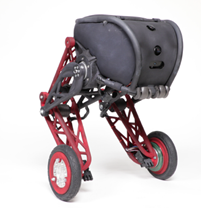
\includegraphics[width=0.4\textwidth]{figures/eth_1.png}
  \hspace{1cm}
  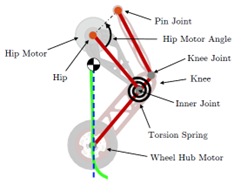
\includegraphics[width=0.4\textwidth]{figures/eth_2.png}
  \caption{Ascento机器人实物图（左）与简化图示（右）}
  \label{fig:eth-ascento}
\end{figure}
腾讯 AI Lab 及 Robotics X 实验室主任张正友博士在机器人行业顶会 ICRA 2021 做大会报告，分享了研发中的轮腿式机器人Ollie\cite{wang2021balance}，在视频中表现了双轮平衡、多模态移动、跳跃、360度空翻等运动能力。Ollie单腿采用并联机构，与身体形成五连杆结构，使整体具有结构简单、动态性能高、爆发力强的特点。机器人基本运动控制采用LQR控制器，此外为适应更多复杂场景，补充采用了IDA-PBC（interconnection and damping assignment- passivity-based control）。

\begin{figure}[H]
  \centering
  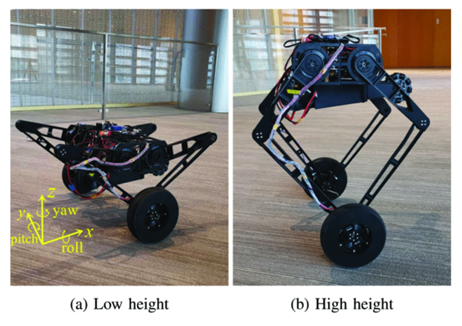
\includegraphics[width=0.5\textwidth]{figures/ollie.png}
  \caption{腾讯AI实验室研发的轮腿式机器人Ollie}
  \label{fig:tencent-ollie}
\end{figure}
\FloatBarrier

\subsection{路径规划算法方案：基于深度强化学习的路径规划算法}

  Tai et al.\cite{tai2016robot}提出了一种基于CNN的DRL模型，该模型以原始RGB-D图像为输入，移动机器人的控制命令为输出。CNN网络的初始权值来自于他们之前工作\cite{tai2016deep}中训练的参数。但是，由于奖励函数的设计没有涉及鼓励探索的机制，因此该模型只能在简单的走廊环境中实现避障。Jiang等人\cite{jiang2019path}提出了一种基于启发式制导和避障知识的DQN算法，在路径规划的训练效率和环境适应性方面取得了一定的效果。然而，由于启发式知识限制了DRL智能体的探索能力，规划的路径在路径长度和平滑度方面并不令人满意。\cite{niroui2019deep}Niroui等人研究了一种将DRL与传统的基于边界的方法相结合的勘探模型。DRL模型输出边界点的权重参数，然后根据预定义的代价函数计算出代价最低的边界点。Chen等人\cite{chen2019self}提出了一种基于DRL的探索方法，该方法以局部网格图为状态空间，动作空间为随机集合。Zhu等人\cite{zhu2022hierarchical}提出了一种分层DRL网络框架，其中低层DRL策略使机器人在向目标位置移动的同时与障碍物保持安全距离，高层DRL策略作为补充，进一步提高路径规划的安全性。同时，通过选择子目标节点减少状态空间，避免稀疏奖励，该方法在采样效率和迁移能力上都取得了出色的表现。
